\section{Related work and back ground}
%ABR video streaming algorithms either choose buffer occupancy \cite{dash:bola,dash:buffer} or both buffer occupancy and current chunk or network throughput \cite{dash:mpc,dash:hotdash,dash:festive,dash:overLTE,dash:smartCache} to select optimal bitrates for future video chunks. Examples would be BOLA \cite{dash:bola} and MPC \cite{dash:mpc}, respectively. Pensieve\cite{dash:pensieve}, HotDASH\cite{dash:hotdash} uses a reinforcement learning (RL) algorithm for optimal bitrate selection to maximize over a QoE metric.

The DASH or DASH like system provides a way (guideline) to change video quality instead of pausing a video streaming during a temporary bad network condition. There are several implementations of the DASH or DASH like video streaming system, and most of them have an HTML5 based implementation using {\it Media Source Extension}(MSE)\cite{wiki:dash,w3c:mse}. Some of these implementations also support {\it Digital Right Management}(DRM) via {\it Encrypted Media Extension}(EME)\cite{w3c:eme}. All the HTML5 based implementations have several modules implemented either in {\it Javascript} or in the browser. The modules like playback, media decryption are implemented in the browser or some browser extension/plugin (\ie Widevine plugin for DRM protection). The different modules are as follows:

{\bf Playback module} or the player is the module that renders a video. It is implemented mostly in the browser. It is mostly implemented in the browser and render in an HTML5 element. The MSE provides the API to access an HTML5 based video player.

{\bf Buffer controller} manages and monitors video buffer. It is partly implemented using javascript and partly by the browser itself. The media contents are stored and decoded by the broswer. A JavaScript module controls the buffer via the available MSE APIs.

{\bf Adaptive bitrate controller} is the module that decides the quality based on the network condition. It can have multiple algorithms and implemented using JavaScript itself. Although it is the most crucial part of DASH like streaming system, it needs to be the most flexible part. Any streaming provider can implement there won algorithm based on their requirement. We discuss more on ABR later part of the article.

{\bf Download manager} is responsible for downloading the segment/chunk chosen by the ABR algorithm. It monitors the progress of ongoing downloads to gain fine-tune information about the network condition. Most of the time, it downloads chunk using AJAX (Asynchronous JavaScript And XML).


{\bf CDN/Streaming Servers} are HTTP based static file server. It contains all the data requires to play a video smoothly.

{\bf DRM protection module:} It provides DRM protection using EME when a streaming provider wants to protect the right of the content. It is an independent component and does not influence the ABR algorithm or other components. The DRM protection module is out of the scope of this work.

\begin{figure}[ht]
	\begin{center}
		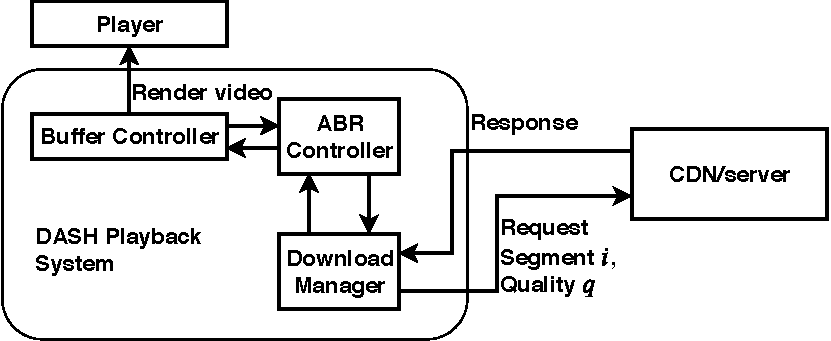
\includegraphics[width=0.7\linewidth]{img/playerDiagram_basic}
	\end{center}
	\caption{\label{fig:playerDiagram_basic} Original DASH based streaming system.}
\end{figure}

The Fig.~\ref{fig:playerDiagram_basic} depict the interconnection between the different module in the DASH bashed players. Here, the ABR controller controls the playback via a buffer controller while instructing the download manager to download the required segment at a suitable time. The ABR controller is the most important component. The ABR controller runs the ABR algorithm with the required information and finds out the quality level or bitrate for the next segment. As the ABR controller is the part of the player, the client application has the implement the ABR controller. In the case of HTML based player, ABRs need to be implemented in JavaScript so that it runs at the viewer's browser. The ABR algorithm like MPC\cite{dash:mpc}, BOLA\cite{dash:bola} or the algorithms described in \cite{dash:probe,dash:cs2p,dash:CFA,dash:rnb,dash:buffer} does not have any special library requirement and can be implemented easily in any technology. However, as machine learning-based, ABR algorithms like Pensieve\cite{dash:pensieve}, OBOE\cite{dash:oboe} or HotDASH\cite{dash:hotdash} need specialized machine learning (ML) library and very hard to implement if the technology does not have support for the required library. So, it is complicated to deploy these algorithms in a browser-based video player.

\begin{figure}[ht]
	\begin{center}
		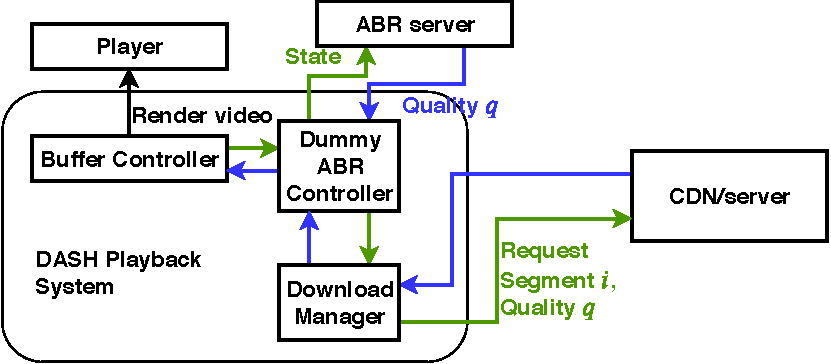
\includegraphics[width=0.7\linewidth]{img/playerDiagram_ml}
	\end{center}
	\caption{\label{fig:playerDiagram_ml} Modified DASH based streaming system to support ML based ABR algorithm}
\end{figure}

Authors of the ML-based algorithm show prototype by modifying the little system bit. The new dash based video system looks like Fig.~\ref{fig:playerDiagram_ml}. Here they propose to replace the ABR controller in the client with a dummy one and run an ABR server in the local system. Every time the player needs to make a decision, the dummy ABR controller contacts the ABR server with the current state of the player. The ABR server responds with the decision based on the algorithm of its choice.

The advantage of this system is that it is independent of client technology. ABR server can be implemented in any technology it suits best. However, it involves extra communication with an external server, which may be fatal to the viewing experience if the round trip time between the player and the ABR server. In the demo, the authors run the ABR server in the client systems to avoid the communication delay between the player and the ABR server. This system is not feasible or scalable to deploy as it needs an ABR server for every player.
